\documentclass[11pt,dvipsnames]{article} % {{{

\usepackage{geometry}
\geometry{total={170mm,240mm}, left=20mm, top=20mm}

\usepackage[utf8]{inputenc}

\usepackage{physics} 
\usepackage{siunitx} 
\usepackage{enumerate} 
\usepackage{pgfplots}
\usepackage{graphicx}
\usepackage{pgfplotstable}
\usepackage{tikz,pgfplots}
\usepackage{amsmath} 
\usepackage{xcolor}
\usepackage{float}
\usepackage{amsfonts}
\usepackage{dsfont}
%\usepackage{bbold}


\newcommand{\fref}[1]{fig.~\ref{#1}}  \newcommand{\tref}[1]{table~\ref{#1}}
\newcommand{\Fref}[1]{Fig.~\ref{#1}}  \newcommand{\Tref}[1]{Table~\ref{#1}}

\newcommand{\h}[1]{\colorbox{Yellow}{#1}}
\newcommand{\1}{\mathds{1}}

\usepackage[]{lineno}  \linenumbers
\setlength\linenumbersep{3pt}
	

\usepackage{fancybox}
\usepackage{colortbl}
\usepackage{amsbsy}
\usepackage[draft,inline,nomargin]{fixme} \fxsetup{theme=color}
\FXRegisterAuthor{cp}{acp}{\color{blue}CP}
\FXRegisterAuthor{ja}{aja}{\color{RedViolet}JA}
% }}}
\begin{document}
% Titulo y otros {{{
\title{Projective maps on a system of $n$ qubits} 
%Title should be concise and to the point  
\author{J. A. de León\\ \small{in collaboration with C. Pineda, D. Davalos, Al Fonseca}}


\date{\today}  

\maketitle
% }}}
% Intro {{{
\janote{en el título: 
así se pone el nombre de Alejo 'Al' o es un typo y debería ir 'A.'?}
According to \cite{bengtsson_zyczkowski_2017}, an arbitrary density matrix on $n$  
qubits can be expanded as
\begin{align}
  \rho = \frac{1}{2^n}\1 + \sum _{i=1}^{2^{2n}-1}\tau _i\sigma _i,
	\label{rho}
\end{align}
where we'll identify $\sigma _i$ as the tensor products of Pauli 
matrices, which form a basis of the space of traceless %\cpnote{Quitar density}
%density 
matrices, and 
$\tau_i$ the projections of $\rho$ onto each element of this particular
basis.

%where the sum is over vectors $\vec{v}=\qty(v_1,\cdots, v_n)$ with entries
%$v_i$ chosen from the set $\{0,1,2,3\}$. We label the coefficients $\Tr \qty(
%\sigma _{v_1} \otimes \sigma_{v_2} \otimes \cdots \otimes \sigma_{v_n}
%\rho )$ as $r_{v_1, v_2,\ldots, v_n}$ to shorten the notation. 


In this work, we are interested in studying the set of maps that erase
some components $\tau_i$ in $\rho$ and characterize the subset of maps
that are quantum channels. We'll refer to the coefficients in both terms of 
\eqref{rho} as the components in $\rho$. 
\cpnote{Quiza vale la pena poner uno o dos ejemplos acá.} 
\janote{\h{Inicio}}
For 1 qubit the picture of our problem is easy to understand given that 
$\tau_i$ are the components of a vector in the Bloch ball, the so-called
Bloch vector. As an example
of a map of our interest let's consider one that erases any of the 
components of the Bloch vector. Geometrically, this map collapses 
the Bloch ball into a disk. This kind of map results not to fulfill 
the completely positive condition.  
\janote{\h{Fin.}}

%The kind of maps that act on density matrices of the form \eqref{rho} that
%we're interested in are those which leave invariant or erase  
%components
%in $\rho$ (i.e. $r'_{v_1, v_2,\ldots, v_n}=r_{v_1, v_2,\ldots, v_n}$ or
%$r'_{v_1, v_2,\ldots, v_n}=0$, where the primed $r$'s refer to the 
%components in the transformed density matrix $\rho '$). 

So far, with a numerical method we've characterized all 1 and 2 qubit maps, 
whereas for 3 qubits system we have numerically analized only maps that leave 
invariant 1, 2, 3, 4, and 64 components in $\rho$. Nonetheless, we have strong
indications that point that only the maps that leave invariant 8 components are 
needed to analyze in order to find the complete set of 3-qubit quantum 
channels.
% }}}
\section*{Results} % {{{
\janote{Modifiqué este párrafo y agregué el cubo para 3 qubits en
la fig 1, porfa revísalo}
In \fref{fig:pictorial-rep-rho} we introduce a pictorial representation 
of an arbitrary density matrix for a system of 1, 2 and 3 qubits. It 
will be useful to visualize the kind of maps of our study making use
of this tool. We'll consider any little square or cube in blank
as a component erased in $\rho$ by the map.
\begin{figure}[H] % {{{
	\centering
	\hfill \hfill
	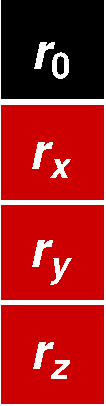
\includegraphics[height=2.5cm]
	{img/tablero-1q}
	\hfill
	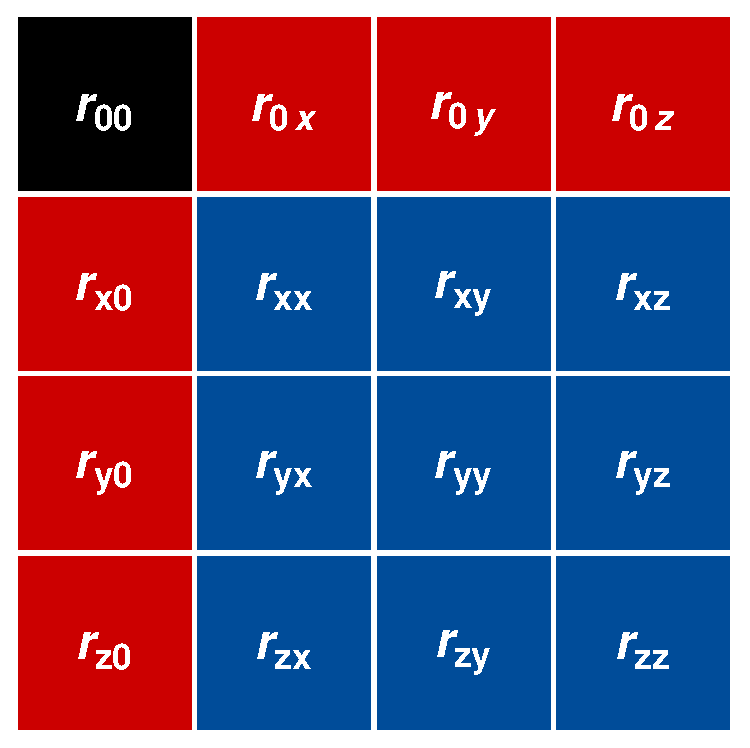
\includegraphics[width=2.5cm]
	{img/rho2q(2)}
	\hfill 
	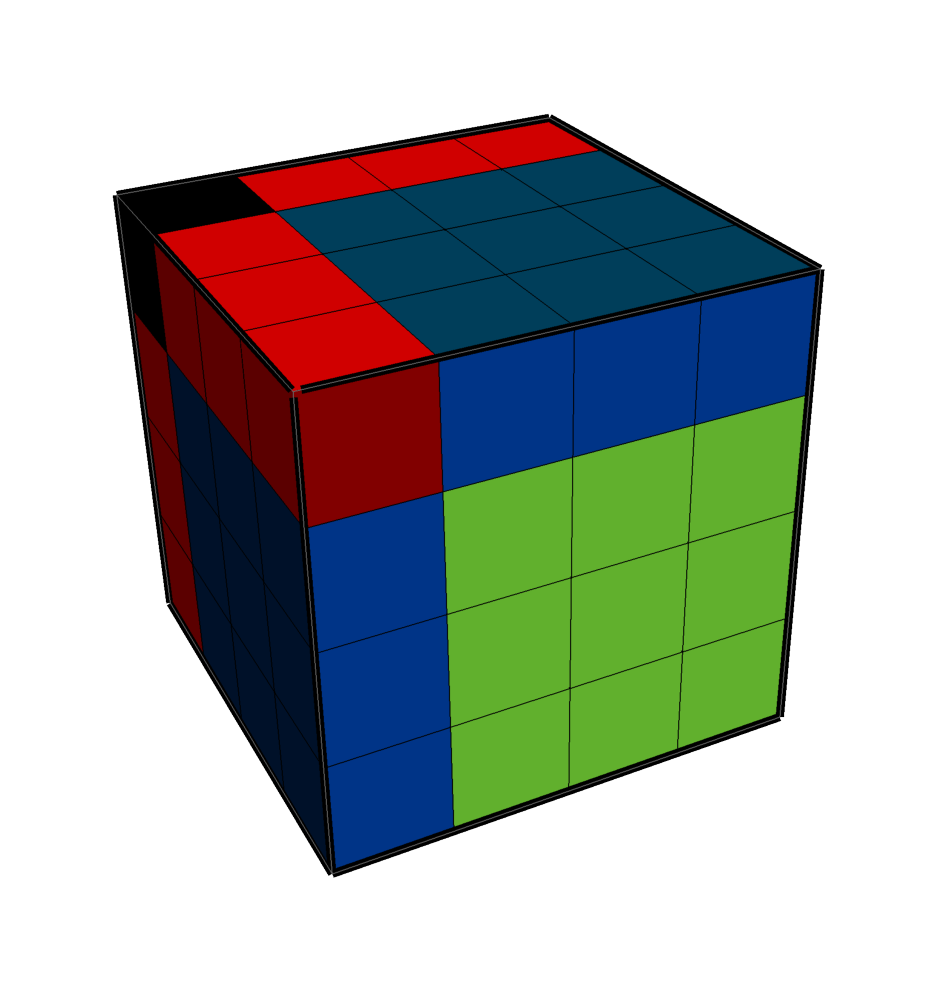
\includegraphics[width=2.5cm]
	{img/rho-3q}
	\hfill \hfill
	\caption{From left to right a pictorial representation for an arbitrary
	density matrix for 1, 2 and 3 qubits, respectively. 
	Red squares refer to components of local Bloch vectors,
	blue squares to correlations between any pair of qubits and
	green squares to correlations between all qubits in the system, for
	the 3-qubits case.}
	\label{fig:pictorial-rep-rho}
\end{figure} % }}}
In the following subsections we show the density matrices that result from
applying a quantum channel to an arbitrary density matrix in the representation
of Figure \ref{fig:CCs-by-components}.

\subsection*{1 qubit} % {{{
\begin{figure}[H]% {{{
	\centering
	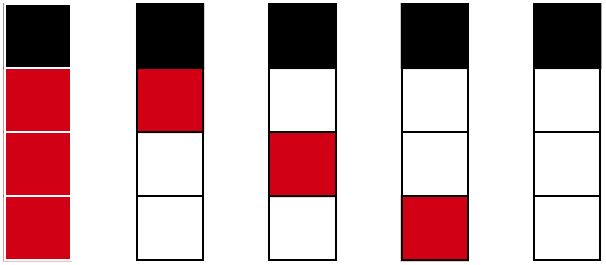
\includegraphics[width=5cm]
	{img/1q-CCs.png}
	\caption{\cpnote{Acá mas bien estas dibujando los canales. Claro queu
se pueden interpretar como matrices, pero mejor dejar que estos diagramas
definan canales. Si no, creo que puede causar confusion. } 1-qubit 
quantum channels.
\janote{Listo.}
}
	\label{fig:1q-ccs}
\end{figure} % }}}
\cpnote{Creo que sería bueno decir algo de los resultados de un qubit. Tener una sección sin nada de texto 
es medio chistoso. Igual comenta a que corresponde cada uno de los canales. Todos esos tienen nombre propio.
Creo que se puede tambien notar el número de componentes que deja invariante
ese bicho. También están organizados en clases de equivalencia.}
\janote{\h{Inicio}}
The first and last channels in \fref{fig:1q-ccs} are the identity and the
completely depolarizing. In between them, from left to right, the 
channels are
the bit-phase flip, phase-flip and bit-flip,
respectively, all of them for the particular 
case $p=0.5$.	This last three channels are equivalent via permutation
of the components $\tau_i$ of the Bloch vector in \eqref{rho}.
\janote{\h{Fin}}
% }}}
\subsection*{2 qubits} % {{{
2-qubit results have been classified in equivalence classes (as shown
from \fref{fig:2q-c1} to \fref{fig:2q-c16}) such
that elemtens in a class are conected by
\begin{enumerate}
	\item Transpositions (particle swaps)
	\item Permutations of rows or columns 1-3 (permutation of individual 
	components)
\end{enumerate}
\begin{figure}[H] % {{{
	\centering
  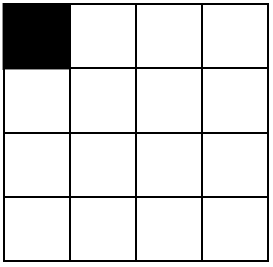
\includegraphics[height=1.2cm]
	{img/C16.png}
	\caption{C${}^{1}$}
	\label{fig:2q-c1}
\end{figure} % }}}

\begin{figure}[H] % {{{
	\begin{minipage}[c]{0.5\textwidth}
		\centering
	  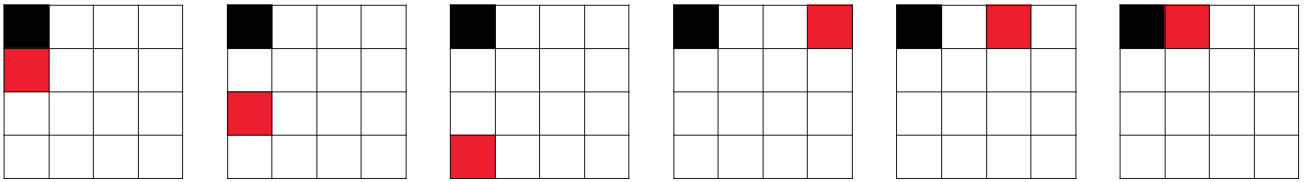
\includegraphics[width=.9\textwidth]
		{img/C12.png}
		\vspace{1.2cm}
		\caption{C${}_1^2$}
	\end{minipage}\hfill
	\begin{minipage}[c]{0.5\textwidth}
		\centering
	  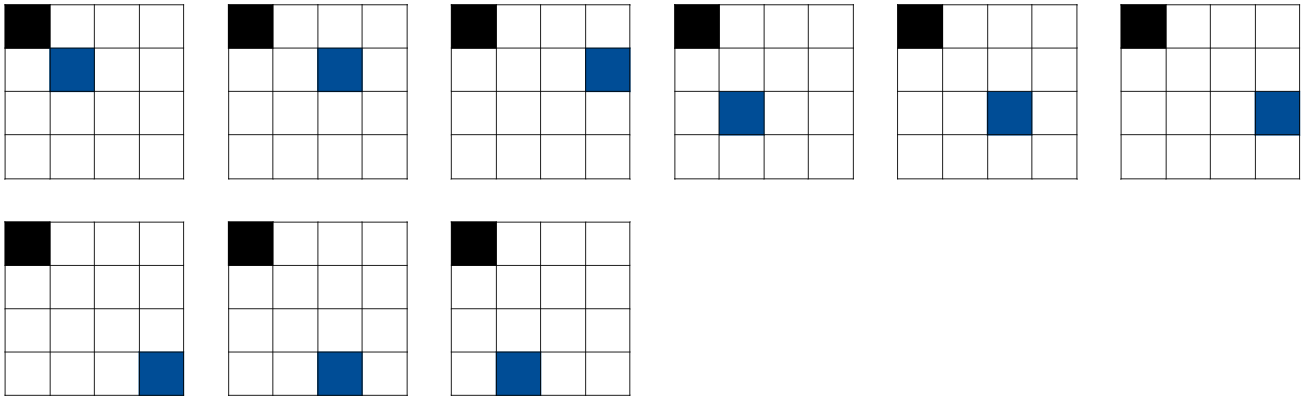
\includegraphics[width=.9\textwidth]
		{img/C22.png}
		\caption{C${}_2^2$}
	\end{minipage}
\end{figure} % }}}

\begin{figure}[H] % {{{
	\begin{minipage}[c]{0.5\textwidth}
		\centering
	  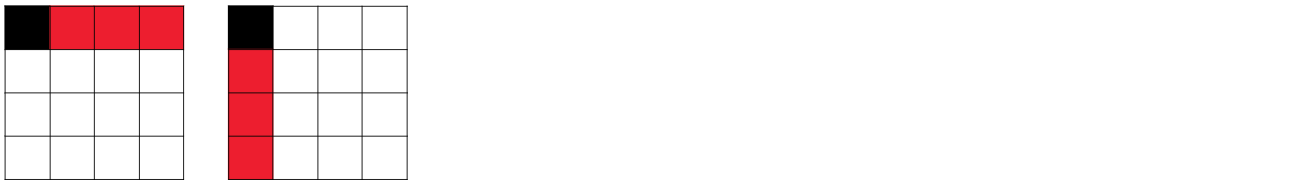
\includegraphics[width=.9\textwidth]
		{img/C14.png}
		\vspace{1.2cm}
		\caption{C${}_1^4$}
	\end{minipage}\hfill
	\begin{minipage}[c]{0.5\textwidth}
		\centering
	  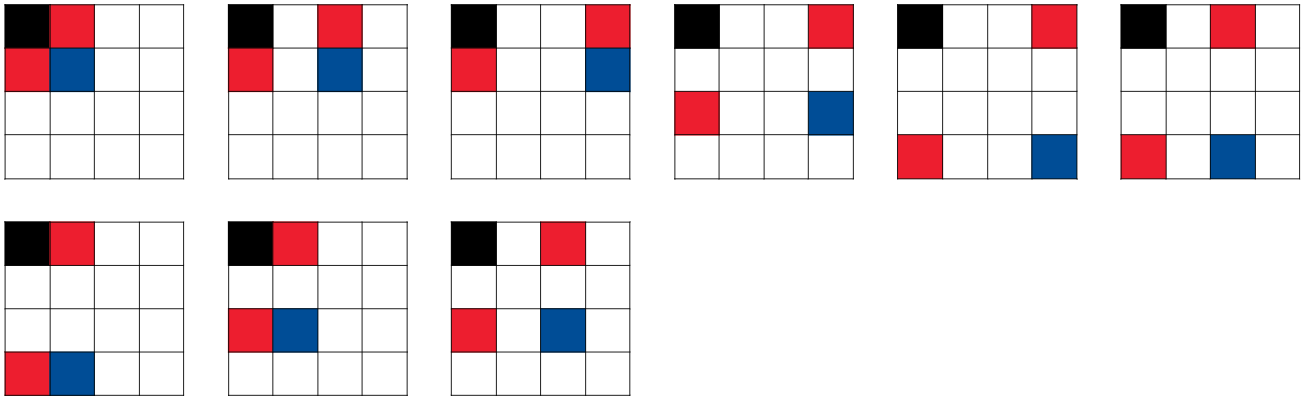
\includegraphics[width=.9\textwidth]
		{img/C24.png}
		\caption{C${}_2^4$}
	\end{minipage}\vfill
\begin{minipage}[c]{0.5\textwidth}
		\centering
	  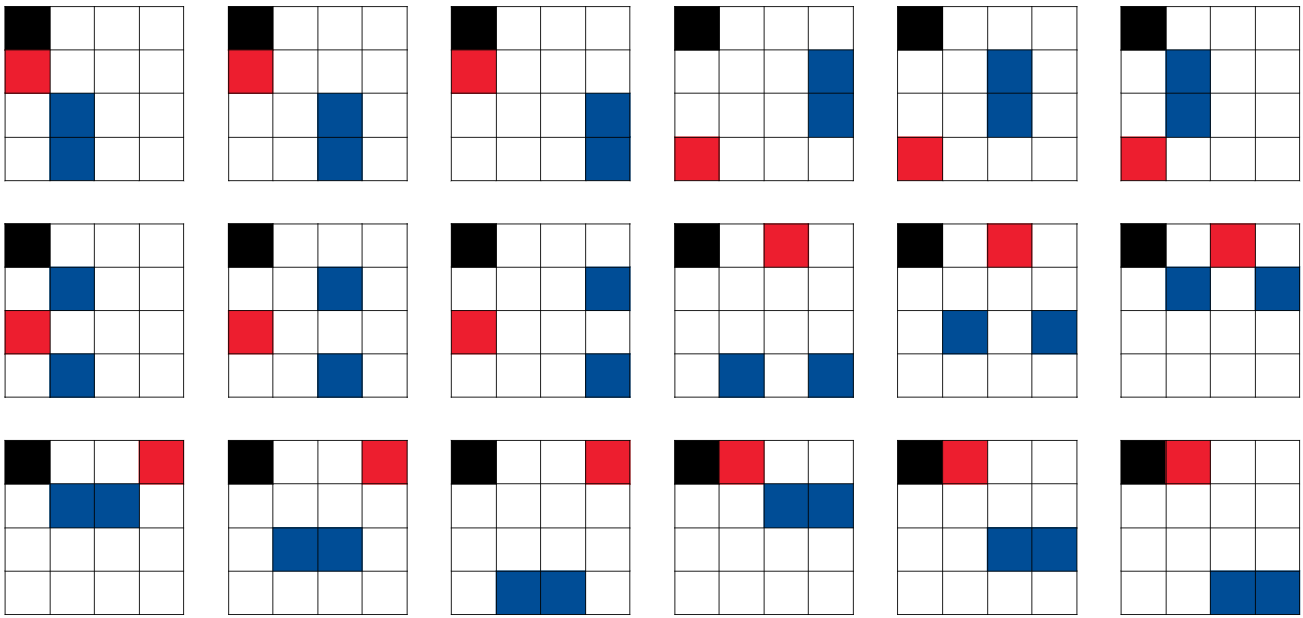
\includegraphics[width=.9\textwidth]
		{img/C34.png}
		\caption{C${}_3^4$}
	\end{minipage}\hfill
	\begin{minipage}[c]{0.5\textwidth}
		\centering
	  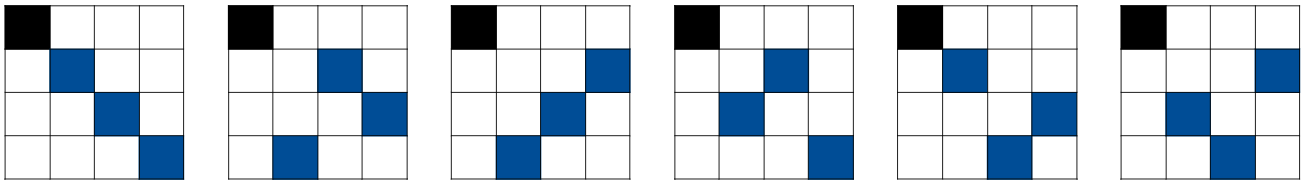
\includegraphics[width=.9\textwidth]
		{img/C44.png}
		\vspace{2.5cm}
		\caption{C${}_4^4$}
	\end{minipage}
\end{figure} % }}}

\begin{figure}[H] % {{{
	\begin{minipage}[c]{0.5\textwidth}
		\centering
	  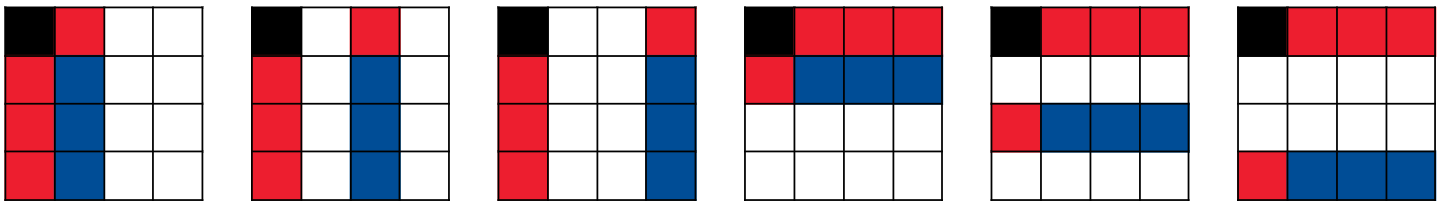
\includegraphics[width=.9\textwidth]
		{img/C18.png}
		\vspace{1.2cm}
		\caption{C${}_1^8$}
	\end{minipage}\hfill
	\begin{minipage}[c]{0.5\textwidth}
		\centering
	  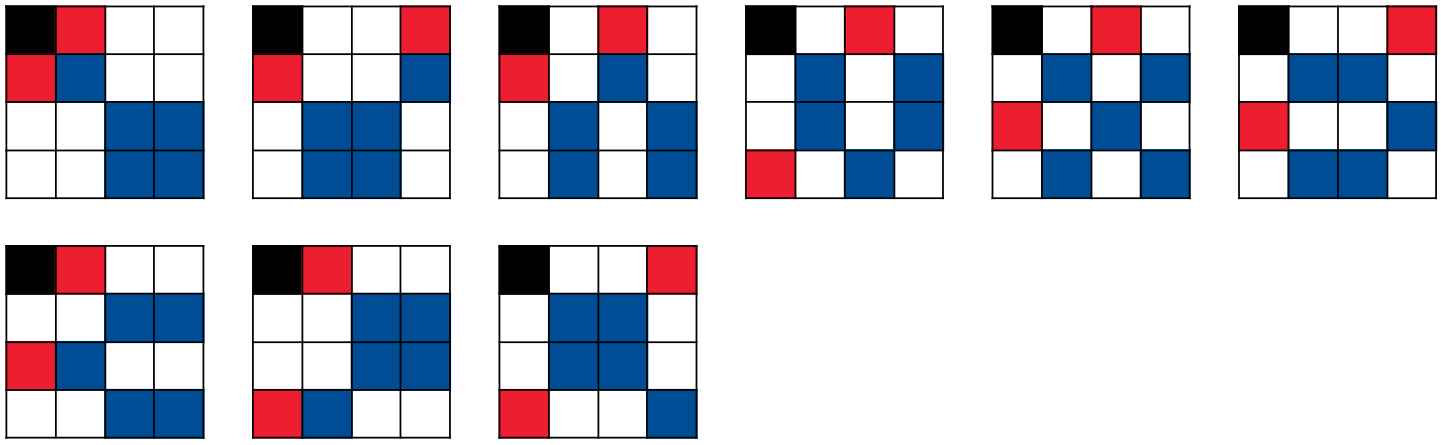
\includegraphics[width=.9\textwidth]
		{img/C28.png}
		\caption{C${}_2^8$}
	\end{minipage}
\end{figure} % }}}

\begin{figure}[H] % {{{
	\centering
  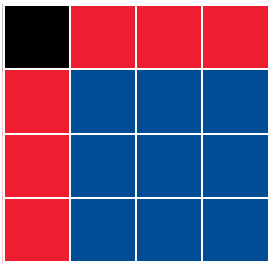
\includegraphics[height=1.2cm]
	{img/C0.png}
	\caption{C${}^{16}$}
	\label{fig:2q-c16}
\end{figure} % }}}

In general, our results exhibit the following features:
\begin{itemize}
\item Only a power-of-2 number of components in $\rho$ 
may be left invariant by quantum
channels. However, not only the number of components in $\rho$ 
to leave invariant is taken into account but actually 
which components are left invariant too.
\cpnote{No entendí esa última frase}
\janote{Quiero decir que no todos los mapeos que dejan un numero de
componentes invariantes igual a una potencia de 2 son canales. Corrijo:}
However, not all maps that leave $2^{k}$ components invariant in $\rho$
are quantum channels. For example, the pattern below corresponds 
to a map that is not a quantum channel. 
\begin{figure}[H]
	\centering
	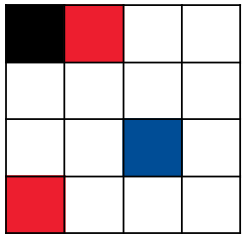
\includegraphics[height=2cm]{img/not-cc}
\end{figure}

\item 
The number of valid quantum channels according to the number of components
left invariant are shown in Figure \ref{fig:CCs-by-components} \fref{fig:CCs-by-components}\cpnote{A mi me gusta 
dejar esto como un comando solo, la referencia a la figura, para poderlas cambiar 
rápidamente y también porque se usa mucho. Checa el codigo acá y en la linea 22 
de este \TeX}. \janote{Listo.}
%Two numbers
%of same color correspond to quantum channels that we suspect have a 1:1 
%correspondence. In the next item we extend this discussion.

\begin{figure}[H]% {{{
	\centering
	\begin{tabular}{>{$n=$}l<{\hfill}*{12}{c}}
1 &&&&&\colorbox{Apricot}{1}&3&\colorbox{Apricot}{1}&&&&&5\\
2 &&&&\colorbox{CadetBlue}{1}&\colorbox{Cyan}{15}&35&\colorbox{Cyan}{15}&\colorbox{CadetBlue}{1}&&&&67\\
3 &&&\colorbox{SpringGreen}{1}&\colorbox{RedOrange}{63}&\colorbox{Yellow}{651}&?&\colorbox{Yellow}{¿651?}&
\colorbox{RedOrange}{¿63?}&\colorbox{SpringGreen}{1}&&&?
\end{tabular}
\caption{First column shows the number of qubits in the system.  In the second
column each position correspond to the number of components invariant ($2^0,
2^1, \ldots, 2^{2n}$) and the numbers shown are the number of quantum channels
according to the number of components invariant.  Finally, third column
specifies the total number of quantum channels for a $n$-qubit system.}
\cpnote{Cambia a $n$-qubit, nota que acá la n es en formato de formula}
\janote{Listo}
\label{fig:CCs-by-components}
\end{figure} % }}}

\item Empirical observations of 2-qubit results led us to some rules that the
patterns in \fref{fig:2q-c1} to \fref{fig:2q-c16} obey:
\cpnote{quizá acá diagrams en vez de figures?} 
\janote{es que se me olvidó poner la referencia a las figuras (no me refería
a los tableros como figuras)}
\begin{enumerate}
\item If a component with indices $ij$ is left invariant, then two options are
allowed: \textit{a.} both components with indices $i0$ and $0j$ are left
invariant too, or \textit{b.} both components with indices $i0$ and $0j$ are
erased.
\cpnote{Creo qeu se puede poner un ejemplo de lo que está permitido y lo que no está 
permitido. Nota que puedes poner un includegraphics sin necesidad de usar el figure. 
Eso creo que cumple con el proposito mejor para lo que buscas}
\janote{\h{Inicio}}
Let's take a look at the next example. \newline

\hfill
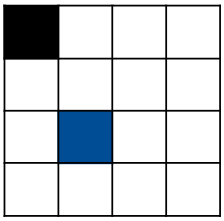
\includegraphics[width=2cm]{img/ex-2q2c-empiricalRule}
\hfill \hfill
\newline
The component with indices 21 in the pattern is left invariant,
so the two options allowed are: \textit{a.} components with indices 01 and
20 are erased, as in this pattern, or \textit{b.} components 
with indices 01 and 20 are left invariant too, 
as in the following pattern \newline

\hfill
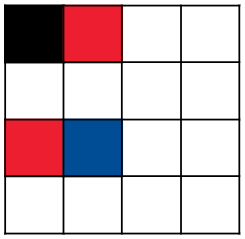
\includegraphics[width=2cm]{img/ex-2q4c-empiricalRule},
\hfill \hfill 
\newline
which is another quantum channel.
\janote{Fin.}

\item Focusing only on the correlation matrix (blue squares): if a component
with indices $ij$ is left invariant and the previous rule is obeyed, then the
remaining components in the correlation matrix on row $i$ and column $j$ must
be erased. 
\cpnote{Tambien una figurita aca o una referencia a algun diagrama estaría padre. 
Si creo uqe mejor referencia a diagramas para no atascar tanto}
\janote{Inicio.}
Let's go back to the last pattern in the previous example. This rule 
ensures that components in the correlation matrix outside of row 2 and 
column 1 may be left invariant by a quantum channel, i.e.\newline

\hfill
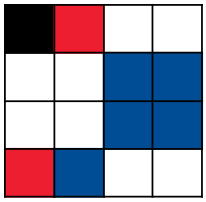
\includegraphics[width=2cm]{img/ex-2q8c-empiricalRule},
\hfill \hfill
\newline
which is another quantum channel.
\janote{\h{Fin}}

\end{enumerate}	
Actually, this two simple rules allow us to connect two elements of classes
C${}^2_k$ and C${}^8_k$. \cpnote{Creo que se pueden hacer más conexiones, no?}
\janote{Es cierto, corrijo:}
Actually, this two simple rules allow us to `\textit{jump}' between
different equivalence classes. In the previous example we were able to connect 
an element of C${}_2^2$ to one of C${}_3^4$, to another one of
C${}_2^8$.



\janote{Agrego el siguiente item porque no le había dado la suficiente
importancia unos items arriba (en el de la fig. 13)}
\item \textit{(Rainbow hypothesis)} Quantum channels
that leave $2^k$ components invariant and $2^{2n-k}$ have a
1:1 correspondence. That is to say, two numbers of the same color 
in \fref{fig:CCs-by-components} correspond to quantum
channels that have a 1:1 correspondence. 

\item The action of a quantum channel on every subsystem must be another
channel. 
\cpnote{Esto también hay que explicar que efecto tiene en los diagramas}
\janote{\h{Inicio}}
This can be seen from the patterns in \fref{fig:2q-c1} to \fref{fig:2q-c16}.
Recall that red squares represent components of local Bloch vectors 
and blue squares represent correlations shared between qubits. 
Then, it may be noted that in the first column and first row of every
pattern there is a 1-qubit quantum channel, of the form of \fref{fig:1q-ccs}.
\janote{\h{Fin}}
\end{itemize}

\subsection*{3 qubits} % {{{
\cpnote{Sugiero que pongas algo de lo que hemos venido haciendo aca. Resultados preliminares. 
Son importantes para la discucion pues lo obvio es comenzar a explorar 3 qubits.}

Recall that for 3 qubits system
we have numerically analyzed only maps that leave 
invariant 1, 2, 3, 4, and 64 components in $\rho$. Therefore,
results presented in this section are preliminary. Quantum channels
follow the same features of 2 qubits system. Not all 3 qubits quantum 
channels
are shown as in the previous section, but only one element of every equivalence
class found. Elements in equivalence classes are connected via particle swaps 
and permutation of individual components.

\subsubsection*{1-invariant-component maps}
The only map that leaves invariant 1 component in $\rho$ is the completely
depolarizing channel.
\begin{figure}[H]
	\centering
	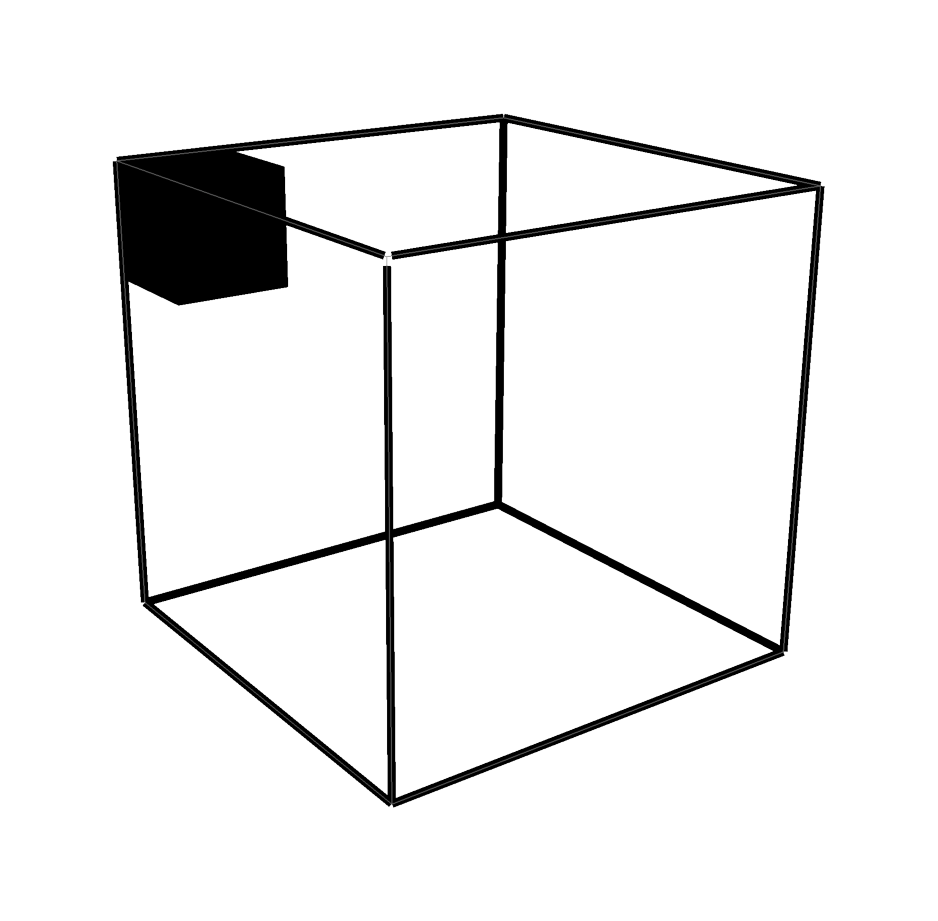
\includegraphics[height=4cm]{img/3q-1c}
	\caption{Completely depolarizing channel for 3 qubits.}
\end{figure}

\subsubsection*{2-invariant-components maps}
All 63 maps that leave invariant 2 components in $\rho$ are 
quantum channels. It's important to mention that in the 2 qubits case all 
2-invariant-components maps are quantum channels, too. There are
3 equivalence classes, quantum channels that leave invariant
\begin{enumerate}
	\item any component of a local Bloch vector,
	\item any correlation between any pair of qubits,
	\item any correlation between all qubits in the system.
\end{enumerate}
\begin{figure}[H]
	\centering
	\hfill \hfill
	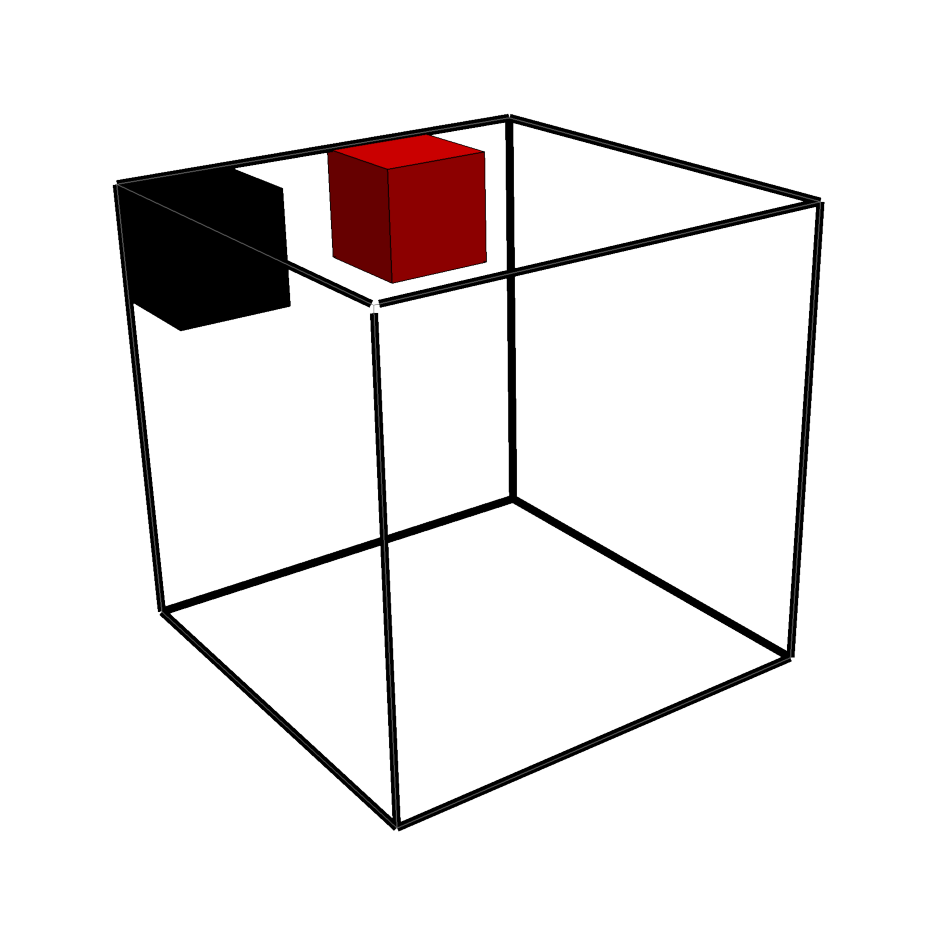
\includegraphics[height=4cm]{img/3q-2c-1}
	\hfill
	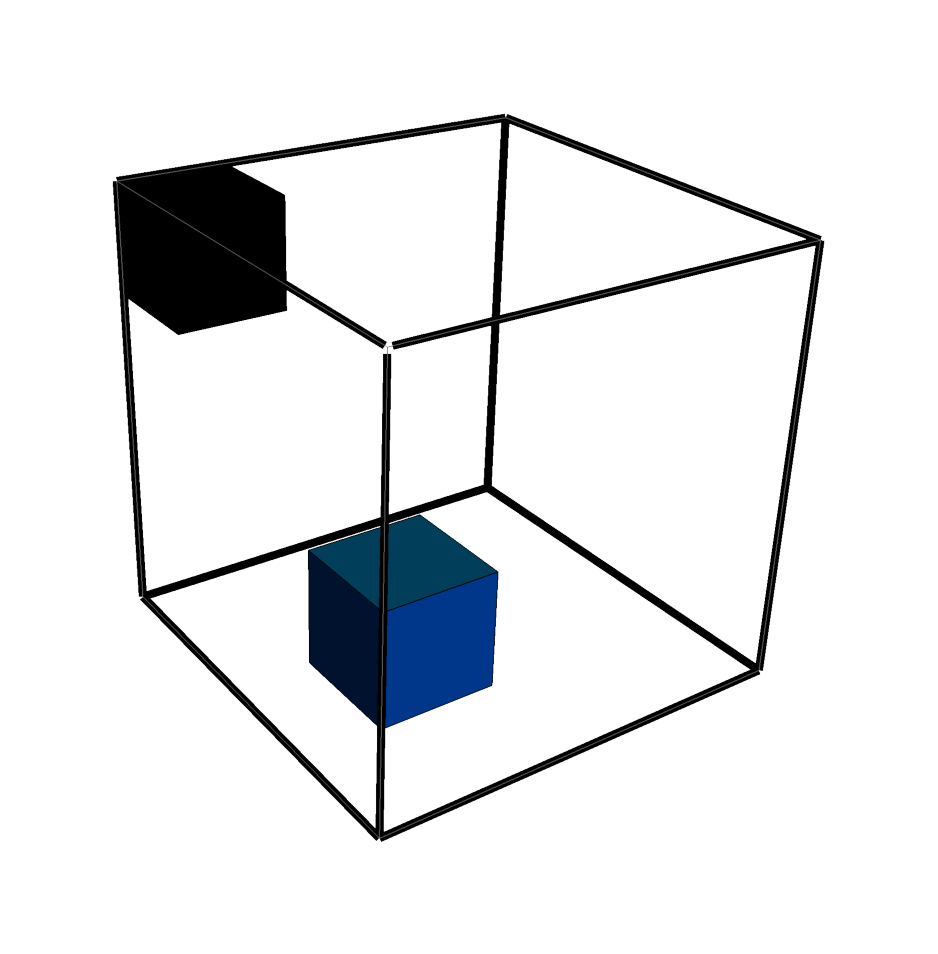
\includegraphics[height=4cm]{img/3q-2c-2}
	\hfill
	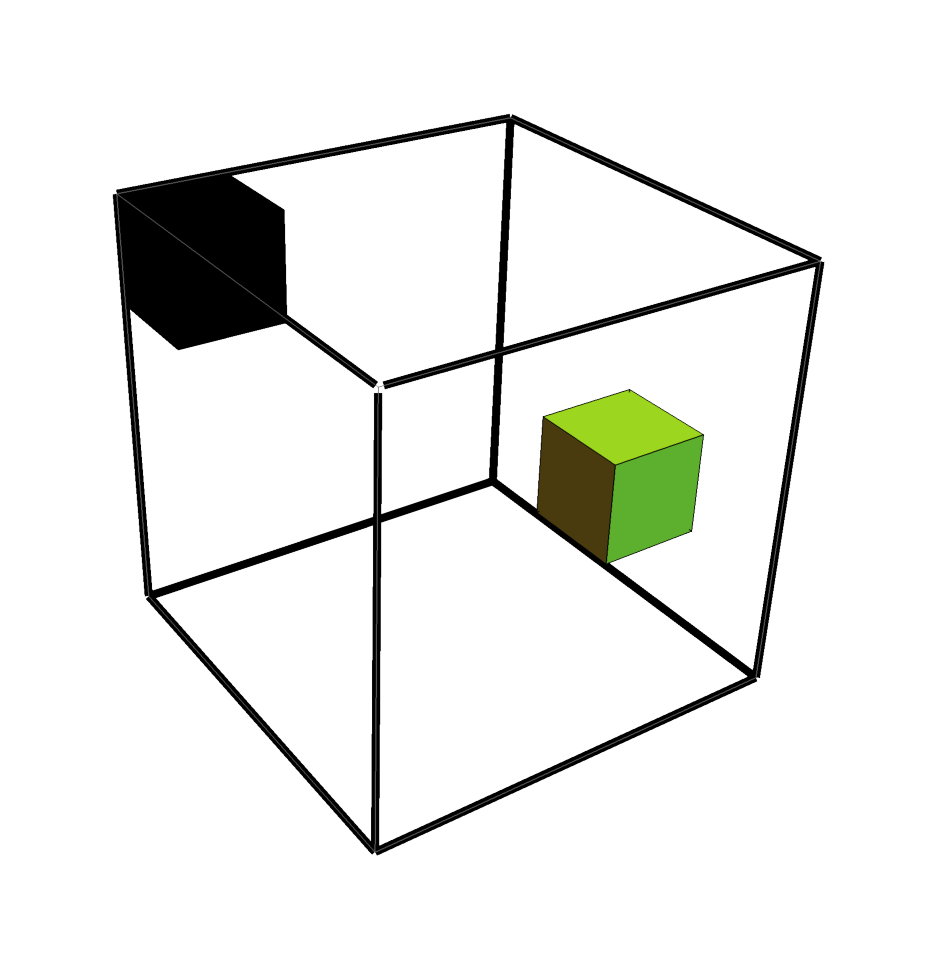
\includegraphics[height=4cm]{img/3q-2c-3}
	\hfill \hfill
	\caption{3-qubits quantum channels. Three equivalence classes 
	(from left to right): leaves invariant one component of any local
	Bloch vector, one correlation between any pair or qubits, and 
	one correlation between all qubits in the system.}
\end{figure}

\subsubsection*{4-invariant-components maps}
There are 39,711 maps that leave invariant 4 components in $\rho$, 651
are quantum channels and may be classified in 10 equivalence classes, as
shown in \fref{fig:QC-3q-4c}.
\begin{figure}[H]
	\centering
	\hfill \hfill
	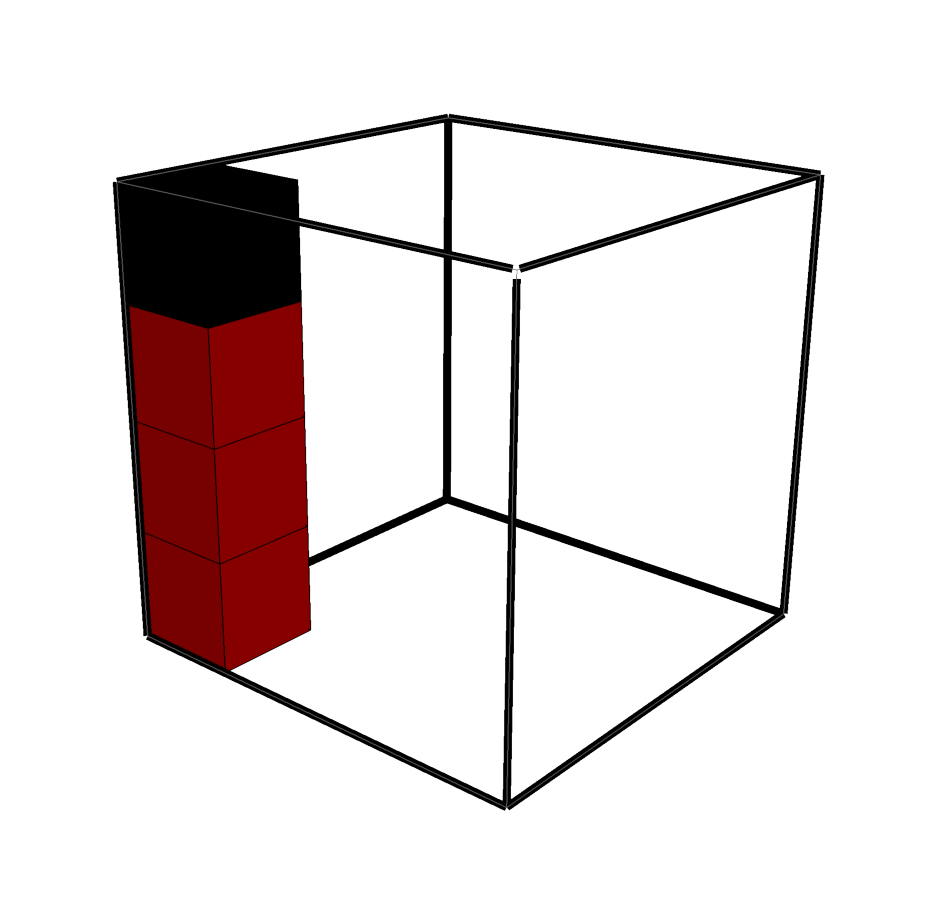
\includegraphics[height=3cm]{img/3q-4c-si-1}
	\hfill
	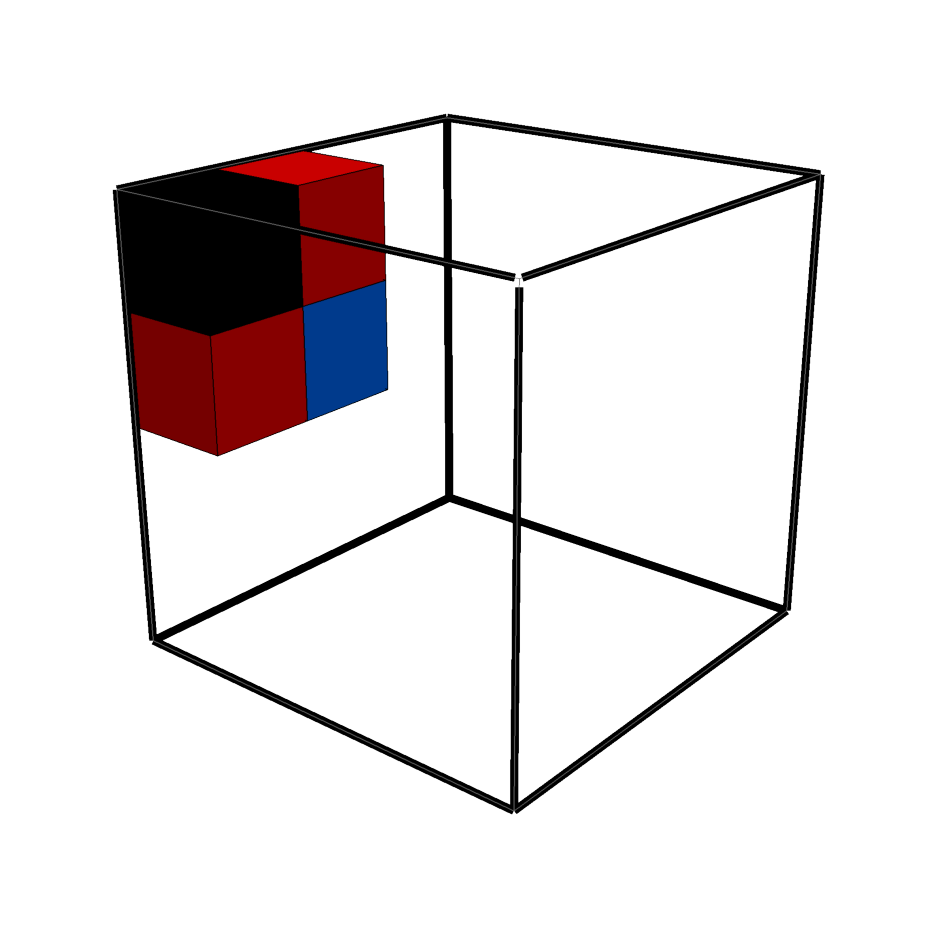
\includegraphics[height=3cm]{img/3q-4c-si-2}
	\hfill
	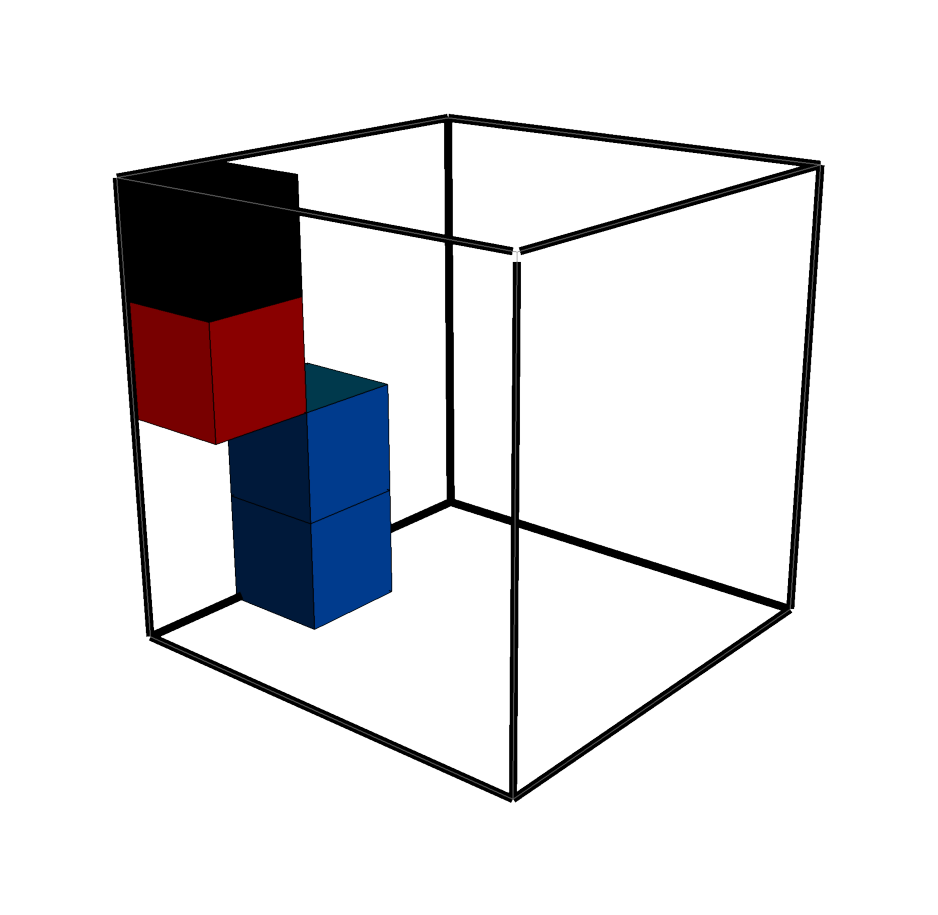
\includegraphics[height=3cm]{img/3q-4c-si-3}
	\hfill
	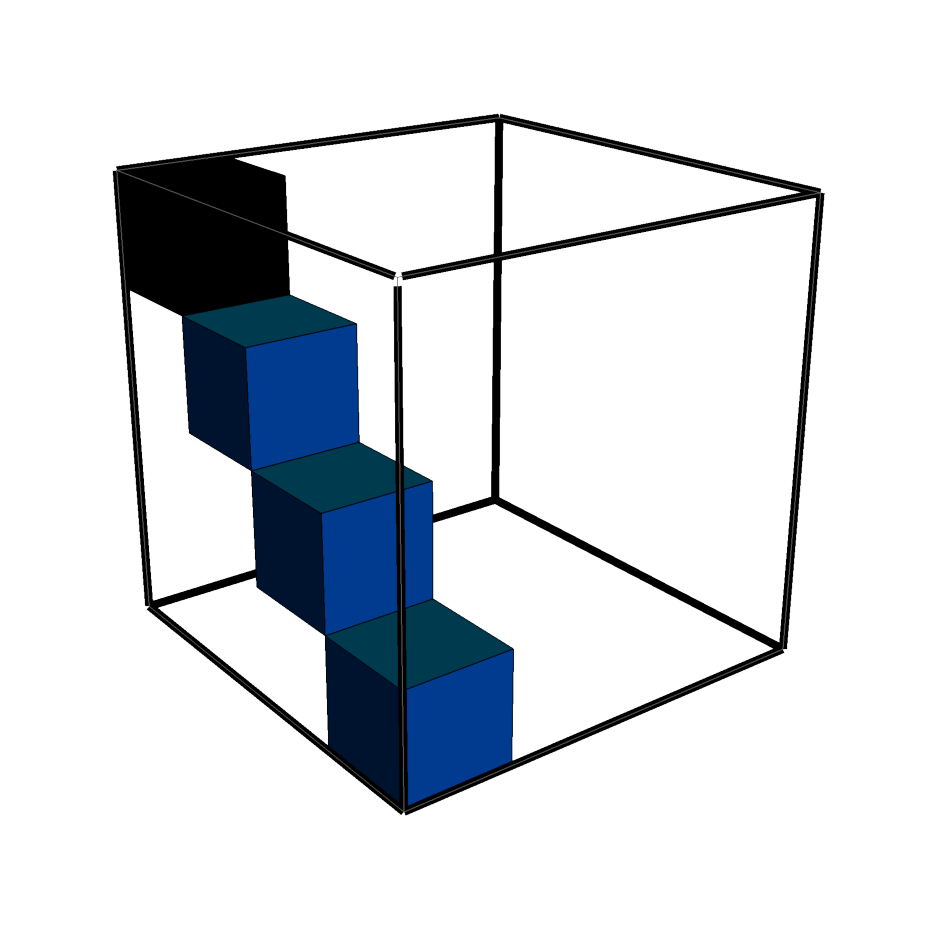
\includegraphics[height=3cm]{img/3q-4c-si-4}
	\hfill
	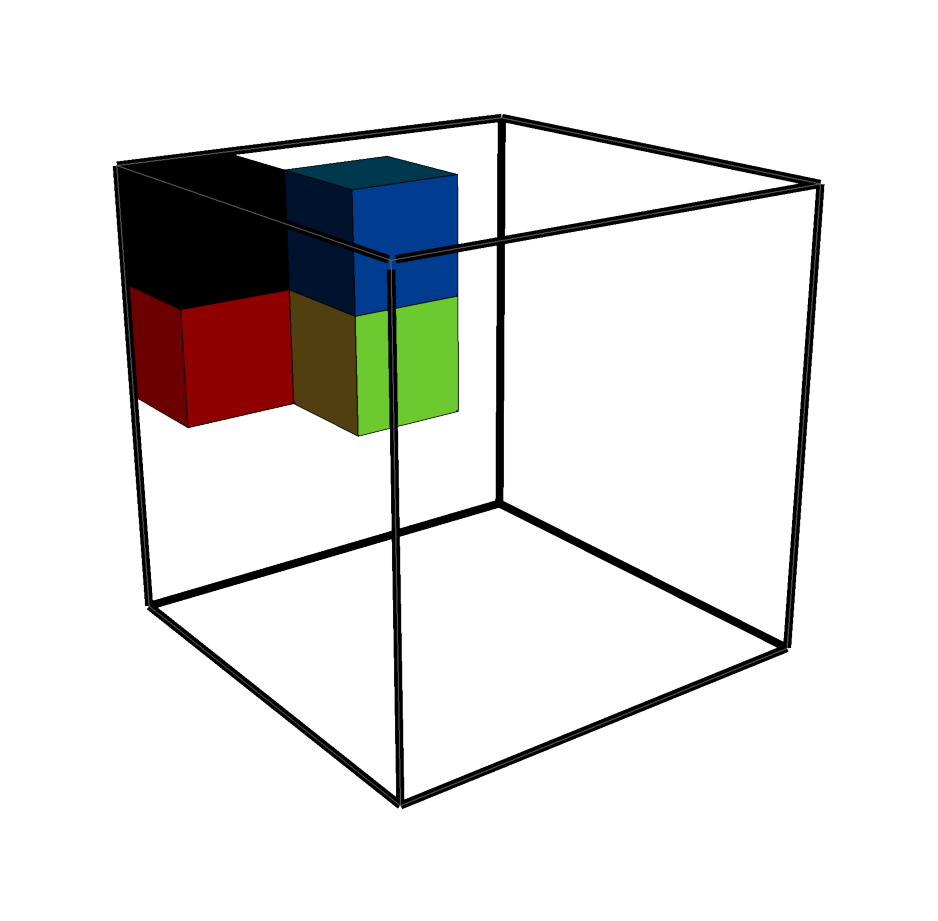
\includegraphics[height=3cm]{img/3q-4c-si-5}
	\hfill
	\vfill
	\hfill
	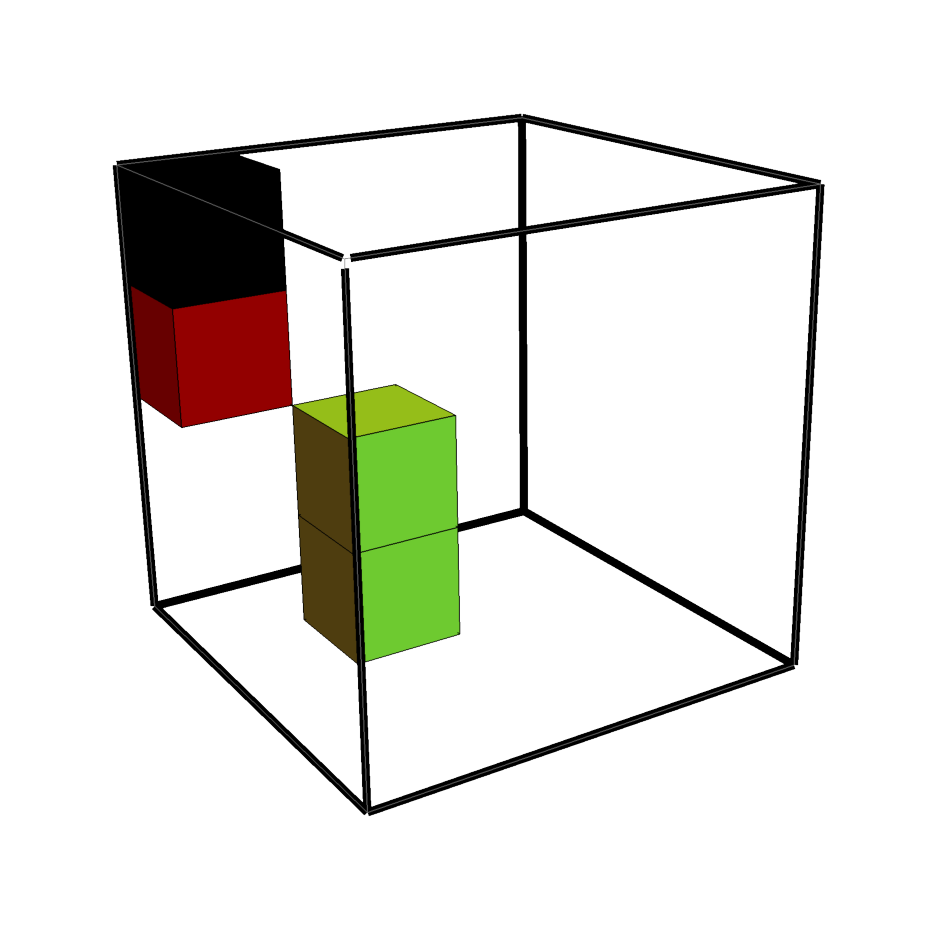
\includegraphics[height=3cm]{img/3q-4c-no-1}
	\hfill
	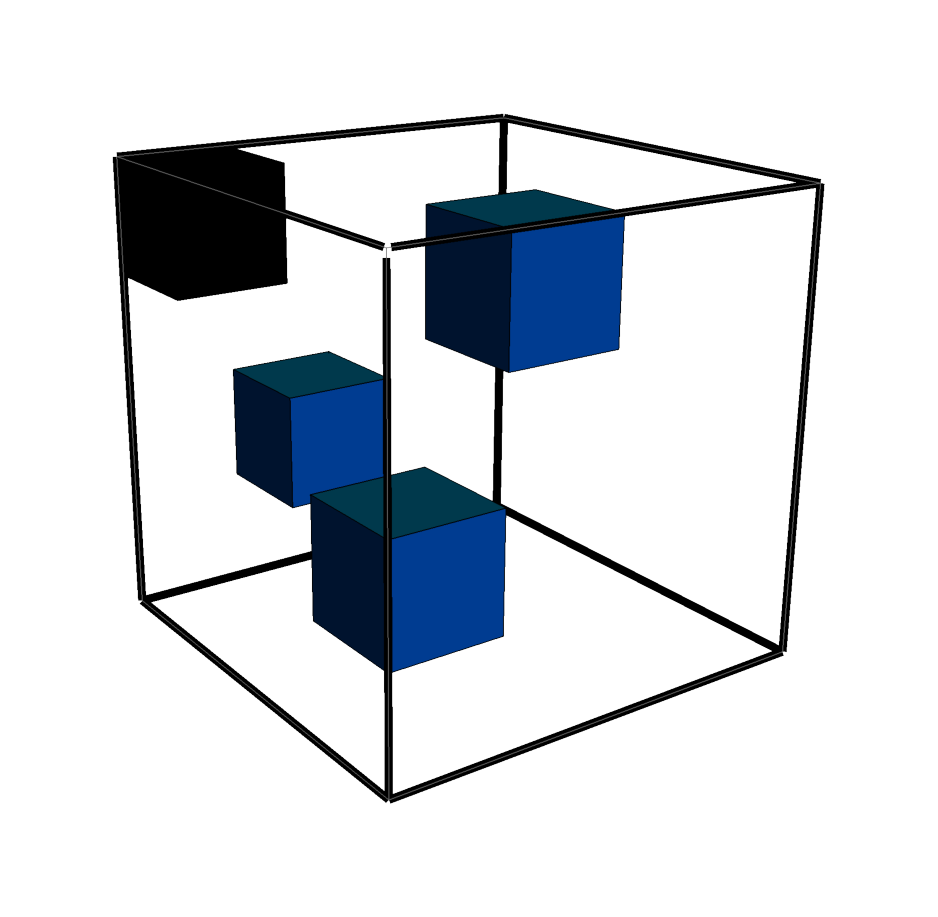
\includegraphics[height=3cm]{img/3q-4c-no-2}
	\hfill
	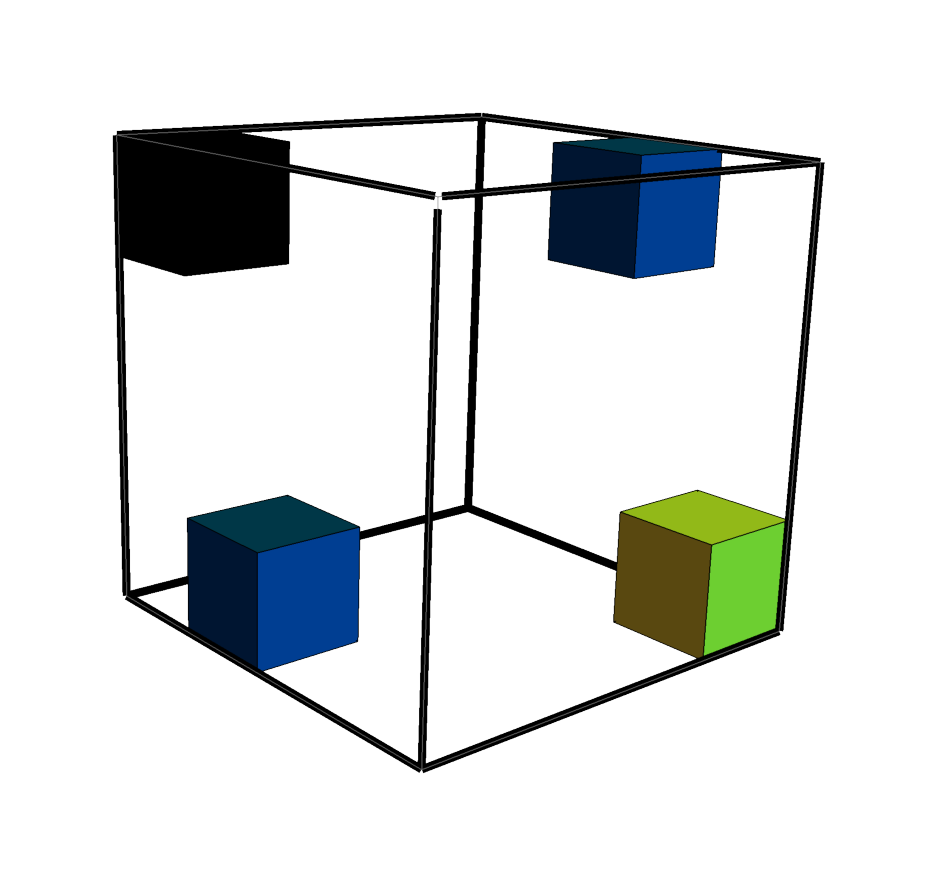
\includegraphics[height=3cm]{img/3q-4c-no-3}
	\hfill
	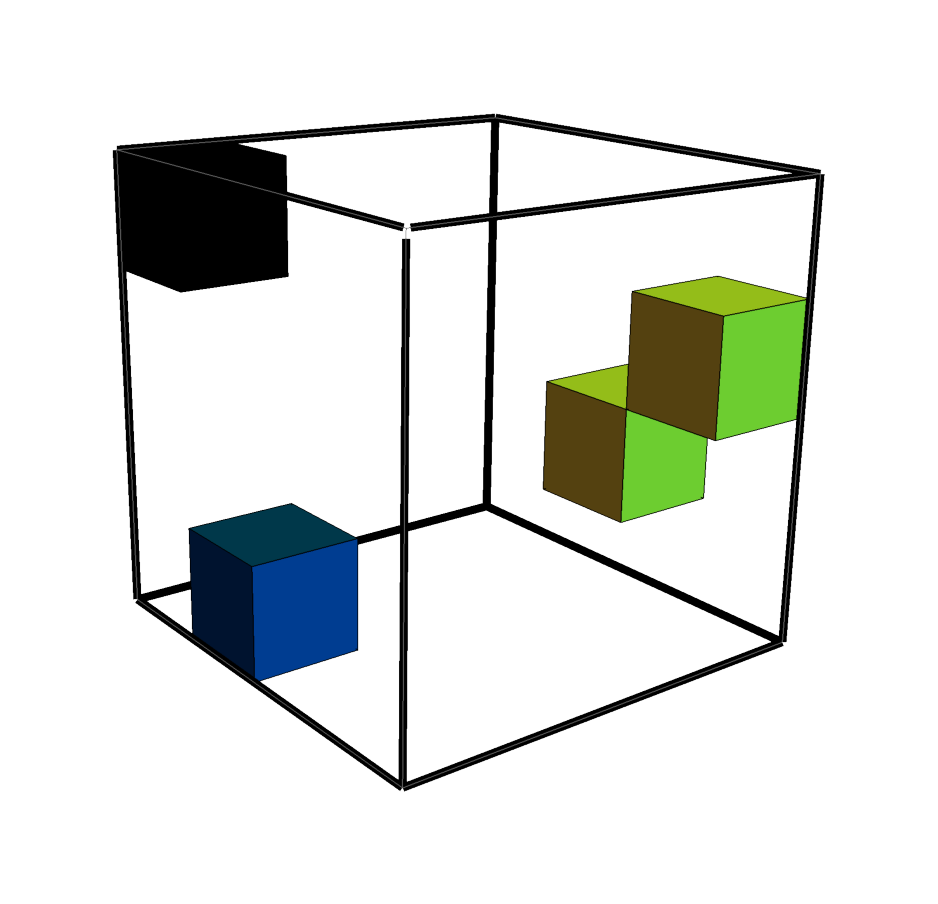
\includegraphics[height=3cm]{img/3q-4c-no-4}
	\hfill
	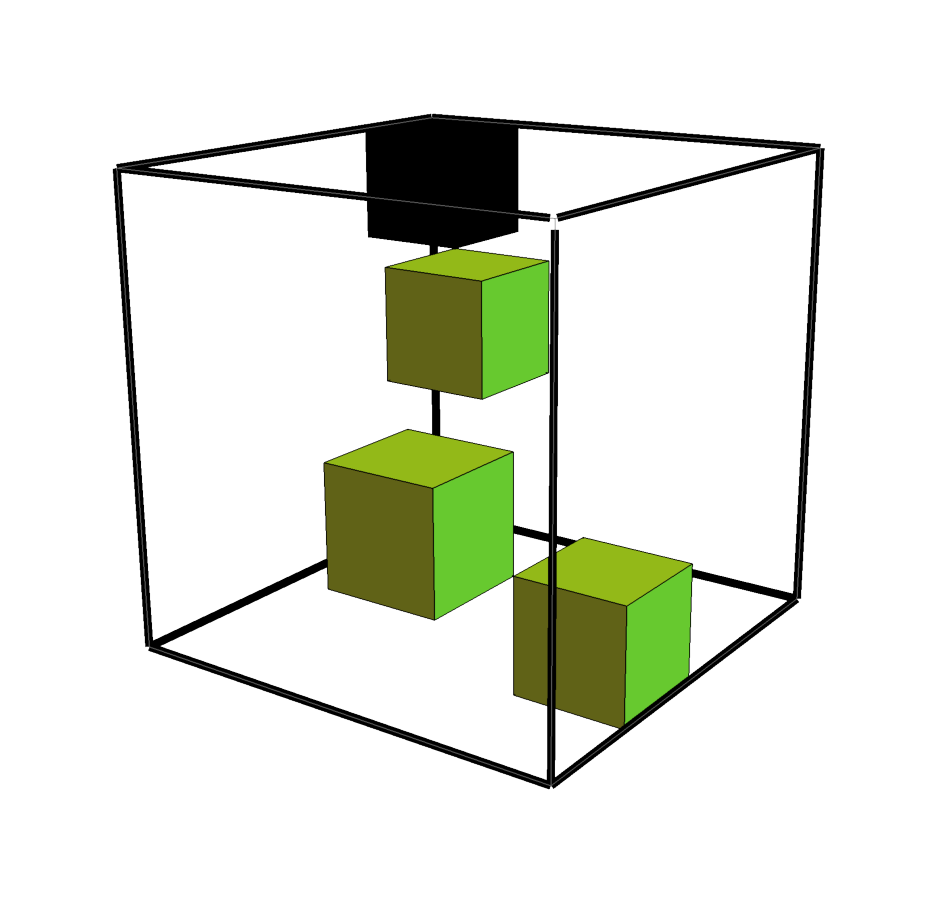
\includegraphics[height=3cm]{img/3q-4c-no-5}
	\hfill \hfill
	\caption{One element of every of the 10 equivalence
	classes of the 3-qubits 2-invariant-components quantum channels.}
	\label{fig:QC-3q-4c}
\end{figure}

\section*{\h{Are this channels a subset of Pauli diagonal channels constant
on axes?}}
\janote{Hola David. Esta es la sección de los mapeos de Ruskai}
%\cpnote{Esto amerita otra sección aparte} \janote{Listo.}

We explored if the quantum channels of our study were a subset 
of Pauli diagonal channels constant on axes \cite{nathanson2007pauli}.
We concluded that not all the set of our channels but only a subset
is contained in the set of Pauli diagonal channels constant on axes.
We'll discuss what a Pauli diagonal channel constant on axes is and 
the argument that led us to the conclusion stated previously.

Let's consider any density matrix written as
\begin{align}
	\rho = \frac{1}{d}\qty[\1 + \sum _{J=1}^{d+1} \sum _{j=1}^{d-1}
	v_{Jj}W_J^j],
	\label{eq:ruskai-rho}
\end{align}
where $d$ is the dimension of the Hilbert space of the system and $W_J^j$ 
are generators of a mutually unbiased bases (MUB) for $\mathbb{C}^{d}$.
Then, the action of a Pauli diagonal channel constant on axes on a 
$\rho$ of the form \eqref{eq:ruskai-rho} is to take 
$v_{Jj}\mapsto (s+t_J)v_{Jj}$. The eigenvalues of a Pauli diagonal channel
are 1 and $\lambda _J=s+t_J$. Note that there are $d+1$ eigenvalues 
$\lambda_J$, and every eigenvalue has degeneration $d-1$. 

In order to construct a channel of ours from a 
Pauli diagonal channel $\lambda_J$ must be equal to one or zero. Our
quantum channels have a power-of-2 rank. On the other hand, 
the rank of a Pauli diagonal channel is $1+3k$ ($k\in \mathbb{Z}^+$,
$1\leq k\leq d+1$),
therefore there are subsets of our quantum channels that can't be  
Pauli diagonal channels. For example, a quantum channel of 2 qubits 
($d=4$) that leaves invariant 8 components in $\rho$ has rank 8, and
there's not a $k$ for which the rank of a Pauli diagonal channel may be 8.


%\cpnote{Creo que eso ya lo teníamos claro. Sería bueno que discutieramos pues 
%me gustaría dar mas seguridades. De hecho tu argumento me parece una prueba, pero quizá
%lo tengamos que refinar. Planeemos una reunion pronto con el resto del combo para ver esto.
%Obvio, creo, si hay intersección, pero no son los mismos.}
% }}}

% }}}
% }}}
\section*{To-do} % {{{
In order to fully understand our results and generalize this kind of maps 
for $n$ qubits we propose the following:
\begin{enumerate}
\item Investigate the Kraus operator representation of this quantum channels.
\item Investigate the Schmidt spectrum of the Choi matrix.
\item Investigate the Jamiolkowski isomorphism to find an equivalence between
CP and the empirical rules listed previously.
\item Use our current results to propose an efficient way to do numerical
analysis to find 3-qubit quantum channels that leave 8 components invariant.
\end{enumerate}
% }}}
\bibliographystyle{unsrt}
\bibliography{references}
\vfill

\end{document}
